\section{Half-Space Local Stokes}
\label{sec:halfspace}

The boundary case is the first place where the formal proof diverges sharply
from an ordinary Euclidean box proof.  A boundary chart has image in a
half-space, not in all of \(\R^{n+1}\).  A local box may touch the boundary
face \(x_0=0\).  The correct local theorem therefore has to see the half-space
geometry, as in classical treatments of manifolds with boundary and
differential forms
\cite{warner1983foundations,abraham1988manifolds,lang1995differential,lee2013smooth}.

\subsection{What the paper proof omits}

In the paper proof, after choosing a boundary chart one often writes a local
coordinate box and applies Stokes.  The intended picture is clear: the lower
normal face is the actual boundary of the manifold, while the other faces are
introduced by the coordinate box and should not contribute if the localized
form is supported away from them.  In a proof assistant, this picture becomes
a family of statements:
\begin{itemize}
  \item the lower normal face is the face with coordinate \(x_0=a_0=0\);
  \item its sign agrees with the outward-normal-first boundary convention;
  \item the upper normal face and the tangential faces are artificial;
  \item the artificial face integrals vanish under a topological support
  condition;
  \item the local analytic assumptions are valid for a box that may touch the
  half-space boundary.
\end{itemize}

The last point is especially important.  It is tempting to require smoothness
on an ambient open neighborhood of the closed box.  That requirement is
natural for interior boxes, but it is not the right boundary hypothesis.  If
the box touches \(x_0=0\), there need not be a chart-target open set in the
ambient Euclidean space containing the closed box on both sides of the
boundary.  The bulk derivative is needed on the open box interior; the boundary
faces need continuity and integrability data.  The formal theorem separates
these assumptions instead of smuggling in an invalid ambient-open condition.

The false theorem shape is therefore:
\[
  \text{closed half-space box }[a,b]\subset U,\quad
  U\text{ ambient open},\quad U\subseteq\text{chart target}.
\]
For a boundary box with \(a_0=0\), this asks the chart target to contain
Euclidean points with negative normal coordinate near the lower face.  That is
not part of the half-space chart.  The correct statement replaces this single
ambient-open condition by separate obligations: open-interior differentiability
for the bulk term, closed-box coefficient regularity for face integrals, and
support control for artificial faces.

\subsection{The half-space primitives}

The half-space layer defines the model set, boundary inclusion, boundary
tangent frame, outward normal, and sign convention.  The relevant names include
\code{upperHalfSpace}, \code{boundaryInclusion},
\code{outwardFirstBoundaryFrame}, and \code{halfSpaceBoundarySign}.
The theorem
\[
\code{halfSpaceBoundarySign_eq_outwardFirstBoundaryOrientationSign}
\]
aligns the coordinate lower-face sign with the outward-first convention used
for the boundary.  Without this bridge, the local lower-face term would remain
a cube face term rather than the represented boundary contribution.

The support box is encoded by \code{halfSpaceSupportBox}.  It is the portion of
the coordinate box that is relevant for the half-space theorem.  The formal
support condition used by local Stokes is expressed through
\[
\code{boxFaceCoeffTSupportInHalfSpaceBox}.
\]
This condition is later obtained from the zero-localized support theorem for
the selected smooth refinement.

Geometrically, \code{halfSpaceSupportBox} is asymmetric.  In the normal
coordinate it allows contact with the lower face \(x_0=0\), because that is
the true boundary.  In the upper normal direction and in all tangential face
directions it is strict, because those faces are artificial.  This is why the
support theorem can both retain the boundary contribution and remove the rest
of the cube boundary.

\begin{theorem}[Half-space compact-support local Stokes]
\label{thm:halfspace-local}
Let \(\alpha\) be an \(n\)-form-valued coordinate representative on
\(\R^{n+1}\), and let \(a\le b\) be box corners with \(a_0=0\).  Suppose the
interior Stokes fields for \((\alpha,a,b)\) are available and the topological
support of \(\alpha\) is contained in the corresponding half-space support box.
Then
\[
  \operatorname{Bulk}_{a,b}(\alpha)
  =
  \operatorname{sgn}_{\partial\HH}\,
  \operatorname{Boundary}_{a,b}^{x_0=0}(\alpha).
\]
In Lean this is the theorem
\code{halfSpaceLocalStokes_compactSupport_of_interiorFields}.
\end{theorem}

This theorem is the local mathematical engine used by the global route.  The
left-hand side is the coordinate bulk integral of the exterior derivative
coefficient.  The right-hand side is not an arbitrary selected face: it is the
lower normal face, transported through the half-space boundary sign.

\subsection{Artificial faces}

The local Euclidean box theorem produces all faces of the box.  For a boundary
chart, only the lower normal face corresponds to the boundary of the manifold.
The remaining terms are collected in
\[
\code{halfSpaceLocalBoundaryRemainder}.
\]
The main cancellation theorem has the schematic form
\[
  \tsupp(\alpha)\subseteq Q(a,b)
  \quad\Longrightarrow\quad
  R_{a,b}(\alpha)=0.
\]
In Lean this is represented by the chain:
\begin{lstlisting}[language=Lean]
boxRemainingFormFaceTerms_eq_zero_of_tsupport_subset_halfSpaceSupportBox
halfSpaceLocalBoundaryRemainder_eq_zero_of_tsupport_subset_halfSpaceSupportBox
\end{lstlisting}
These theorems are where the informal phrase ``the support misses the
artificial boundary'' becomes a checkable proof.  They also explain why the
global theorem needs topological support control, not merely pointwise
ordinary support information.

The proof has a simple mathematical shape.  Euclidean box Stokes first writes
the bulk integral as the sum of all signed face integrals.  The half-space
boundary API identifies the lower normal face with the true boundary term.
For every other face, support containment in the half-space support box gives
disjointness between the face coefficient support and that face, so the
corresponding face integral is zero.  The remaining equality is exactly
\cref{thm:halfspace-local}.

\subsection{Proof sketch of the local theorem}

The local half-space theorem is obtained by factoring the usual box theorem
through three comparison steps.

\paragraph{Step 1: ordinary box Stokes.}
For a coordinate \(n\)-form \(\alpha\) on \(\R^{n+1}\), the Euclidean box
theorem expresses the integral of the coordinate exterior derivative over
\([a,b]\) as a signed sum over all coordinate faces.  This is the analytic
part of the proof closest to standard treatments of integration and geometric
measure theory
\cite{munkres1991analysis,rudin1987real,federer1969geometric,evans1992measure}.
In the Lean development, this is the part delegated to the box-Stokes infrastructure.  The
\code{HalfSpaceBoxInteriorStokesFields} record stores exactly the hypotheses
that this theorem consumes: continuity of signed coefficients on the closed
box, differentiability on the open box away from a countable exceptional set,
integrability of the divergence term, and the equality between the exterior
derivative coefficient and the coordinate divergence integral.

\paragraph{Step 2: identify the lower normal face.}
Because \(a_0=0\), the lower face in the normal coordinate is the model
boundary of the half-space.  The boundary integral layer proves that the
coordinate lower-face term is the half-space boundary form integral, multiplied
by the sign prescribed by the outward-first convention.  This is the content
of the lower-face and \code{halfSpaceBoundarySign} bridge lemmas.

\paragraph{Step 3: erase artificial faces.}
All remaining faces are introduced by the coordinate box.  The support box is
chosen so that a form whose topological support is contained in it has zero
face coefficient on those artificial faces.  Hence the remainder sum is zero.
This is where the global zero-support theorem is consumed by the local layer.

The result is a local theorem whose hypotheses match what boundary charts can
actually provide.  It does not require a closed box to have an ambient open
neighborhood across the boundary.

\begin{center}
\small
\begin{tabular}{p{0.28\textwidth}p{0.34\textwidth}p{0.24\textwidth}}
\hline
Local ingredient & Why it is needed & Lean location \\
\hline
open-interior differentiability & identifies the bulk derivative on the box
interior & open-interior fields \\
closed-box continuity and integrability & makes the box and face integrals
legal & interior Stokes fields \\
lower normal face sign & turns the cube face into the true boundary term &
boundary-sign lemmas \\
topological support in the half-space support region & removes every
artificial face & face-support predicate \\
\hline
\end{tabular}
\end{center}

\subsection{Interior fields}

The record
\begin{lstlisting}[language=Lean]
structure HalfSpaceBoxInteriorStokesFields
    (omega : (Fin (n + 1) -> Real) ->
      (Fin (n + 1) -> Real) [/\^Fin n]->L[Real] Real)
    (a b : Fin (n + 1) -> Real) where
  le : a <= b
  lower_zero : a 0 = 0
  exceptional : Set (Fin (n + 1) -> Real)
  exceptional_countable : exceptional.Countable
  continuous_signedCoeff : ...
  hasFDerivAt_signedCoeff : ...
  integrable_divergence : ...
  bulk_eq_boxIntegral : ...
\end{lstlisting}
packages exactly what the half-space local theorem needs from the Euclidean
box theorem.  The exceptional set and differentiability fields match the
interface of the underlying box-divergence theorem.  The field
\code{bulk_eq_boxIntegral} bridges the mathlib exterior derivative integrand
and the coordinate divergence integrand used by the box theorem.

This record is the point where the formalization makes a mathematical
distinction that a paper proof can blur.  There is no single phrase
``smooth on the box'' that supplies all of these facts in the boundary case.
Some facts live on the open interior, some on the closed box, and some are
a.e. comparisons between two integrands.  Bundling them into
\code{HalfSpaceBoxInteriorStokesFields} gives the exact contract consumed by
local Stokes, after which later constructors prove the fields automatically
for the selected refined representatives.

The theorem
\begin{lstlisting}[language=Lean]
theorem halfSpaceLocalStokes_compactSupport_of_interiorFields
\end{lstlisting}
then turns these fields plus artificial-face support control into the local
compact-support half-space Stokes identity.  The version
\[
\code{HalfSpaceBoxInteriorStokesFields.withRemainder}
\]
keeps the artificial-face remainder visible, while
\[
\code{HalfSpaceBoxInteriorStokesFields.compactSupport}
\]
uses support containment to remove it.

\subsection{From chartwise smoothness to local fields}

The first-principles theorem does not ask the user for
\code{HalfSpaceBoxInteriorStokesFields}.  Those fields are generated by:
\begin{lstlisting}[language=Lean]
CoverIndexedZeroCompactRepresentedStokesIntrinsicInput.
  interiorFieldsOfSelectedSmoothRefinement
\end{lstlisting}
The constructor uses chartwise smoothness of the original form, smoothness of
the selected refined coefficients, and the fact that the selected closed boxes
lie in the self chart transition source.  It constructs open-interior
smoothness fields and then applies
\[
\code{HalfSpaceBoxInteriorStokesFields.ofOpenInteriorSmoothness}.
\]

The mathematical point is that closed-box regularity is proved for the actual
localized coordinate form on the selected box, while bulk differentiability is
used on the open box interior.  This prevents the global theorem from
depending on a false boundary-chart ambient-open hypothesis.

This split is also important for degenerate boxes.  Some coordinate intervals
may collapse during finite refinement.  In such cases, the closed-box
regularity and integrability statements remain meaningful, while the open
interior may be empty or lower dimensional.  The local fields isolate the
measure-theoretic bridge needed by the box theorem so that degenerate and
nondegenerate cases can be handled uniformly by the surrounding constructors.

\begin{figure}[t]
  \centering
  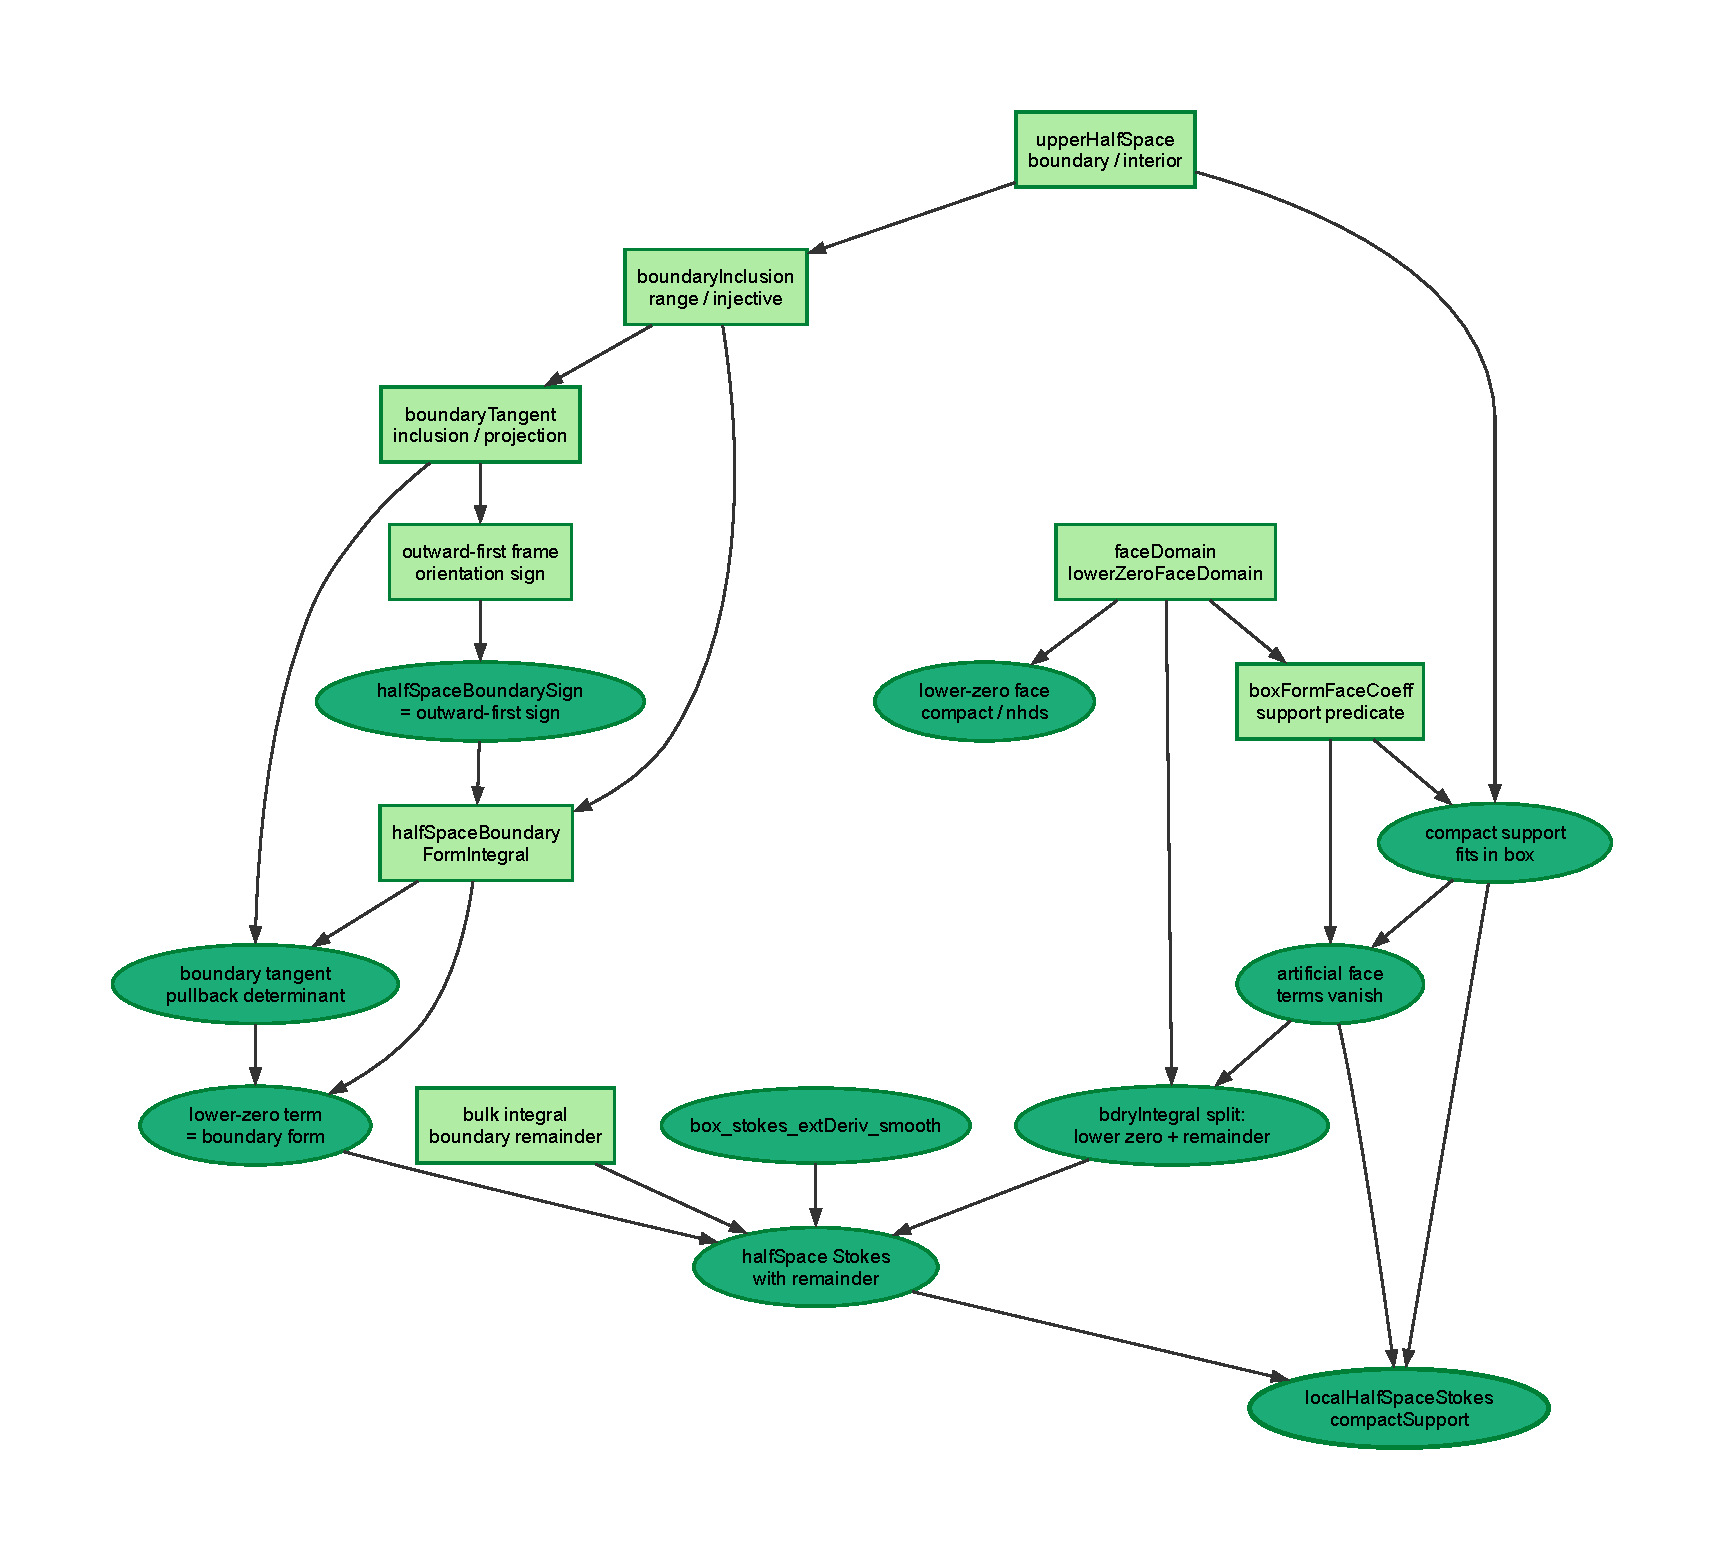
\includegraphics[width=0.86\textwidth]{figures/stokes-halfspace-graph.pdf}
  \caption{The half-space layer separates the true lower boundary face from
  artificial coordinate faces, and separates open-interior differentiability
  from closed-box face regularity.  Light-green rectangular nodes denote
  definitions or constructed data; dark-green oval nodes denote theorem-level
  statements or derived equalities.}
  \label{fig:halfspace-layer}
\end{figure}

\subsection{Why this layer is substantive}

It would be possible to state a global theorem assuming a local Stokes theorem
for every selected box.  The artifact does more: it builds the local theorem
from the half-space box infrastructure and then connects it to the selected
refined representatives.  This is why the final theorem can hide local Stokes
fields.  The local half-space content is not absent from the public API; it is
proved and generated internally.
